
\textbf{Ejemplo 9}\\
El dueño del almacén solicita al banco una aceptación bancaria por 5 millones COP, que
entregará al fabricante o proveedor para que le entreguen la mercancía. El banco presta
este servicio y le cobra al almacén una comisión del 1\% periodo trimestre anticipado sobre
el valor de la aceptación. Considerar el iva del 16\% del valor monetario de la comisión
bancaria.\\
a) Comisión bancaria que debe pagar el almacén por su expedición.\\
Si el fabricante vende la aceptación faltando 40 días a una tasa del 30\% perido días véncido y por ello el
valor de registro en bolsa es de $V_{r}$ = 4.850.000 COP, y la bolsa le hace una retención en la fuente sobre los rendimientos del 7\% calcular: \\
b) El precio de compra Pc incluyendo la retención en la fuente y excluyendo la comisión
del comisionista comprador. \\ 
\textbf{Solución.}
%La tabla ira centrada
\begin{center}
	\renewcommand{\arraystretch}{1.5}% Margenes de las celdas
	%Creación de la cuadricula de 3 columnas
	\begin{longtable}[H]{|p{0.33\linewidth}|p{0.33\linewidth}|p{0.33\linewidth}|}
		%Creamos una linea horizontal
		\hline
		%Definimos el color de la primera fila
		\rowcolor[HTML]{FFB183}
		%%%%% INICIO ASIGNACIÓN PERIODO FOCAL %%%%%%%
		%%%%%%%%%% INICIO TITULO
		%Lo que se hace aquí es mezclar las 3 columnas en una sola
		\multicolumn{3}{|c|}{\cellcolor[HTML]{FFB183}\textbf{1. Asignación período focal}}   \\ \hline
		\multicolumn{3}{|c|} {$pf : 40 pdv$} \\ \hline
		%%%%%%%%%% FIN TITULO
		%%%%% INICIO DECLARACIÓN FORMULAS
		
		%%%%%%%%%%% INICIO TITULO
		\rowcolor[HTML]{FFB183}
		\multicolumn{3}{|c|}{\cellcolor[HTML]{FFB183}\textbf{2. Declaración de variables}}    \\ \hline
		%%%%%%%%%%% FIN TITULO
		%%%%%%%%%% INICIO SUBTITULO
		\multicolumn{1}{|c|}{\cellcolor[HTML]{FFB183}\textbf{Valores monetarios}}    & 
		\multicolumn{1}{|c|}{\cellcolor[HTML]{FFB183}\textbf{Valores no monetarios}} &
		\multicolumn{1}{|c|}{\cellcolor[HTML]{FFB183}\textbf{Incógnitas}}  \\ \hline
		%%%%%%%%%% FIN SUBTITULO
		
		%%%%%%%%%%% INICIO MATEMÁTICAS
		
		$V\textsubscript{r} = 4{.}858{.}285 COP$ & \textit{Com bancaria = 1\%(pta) del valor de la aceptación}& $P_{c} = \% \textit{? COP}$    \\
		
		
		& $R\textsubscript{f} \textit{= 7\% sobre utilidades (F - V\textsubscript{r})}$ & $V_{com} \textit{= ?COP Valor com bancaria}$\\
		&\textit{iva = 16\% de la com bancaria}  & \\
		& \textit{$n = \frac{40}{365} p(40 dv)$}  & \\ \hline
		%%%%%%%%%% FIN MATEMÁTICAS
		
		%%%%% INICIO FLUJO DE CAJA
		\rowcolor[HTML]{FFB183}
		\multicolumn{3}{|c|}{\cellcolor[HTML]{FFB183}\textbf{3. Diagrama de flujo de caja}}                                                                                  \\ \hline
		%Mezclamos 3 columnas y pondremos el dibujo
		%%%%%%%%%%%%% INSERCIÓN DE LA IMAGEN
		\multicolumn{3}{|c|}{ 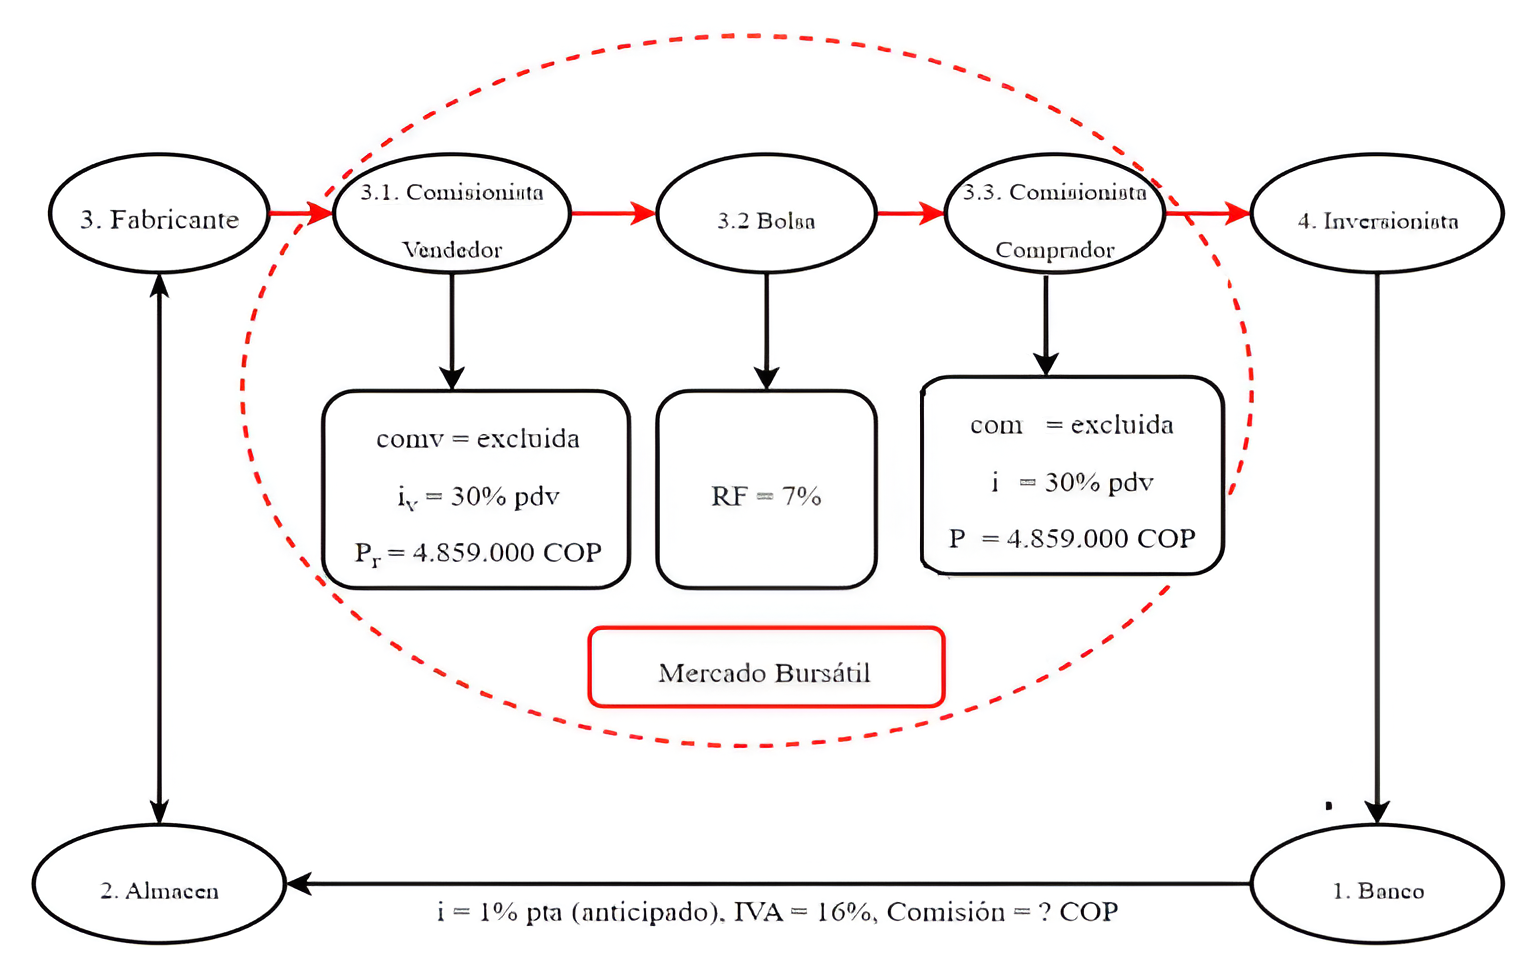
\includegraphics[trim=-5 -5 -5 -5 , scale=0.55, width=16.4 cm, height = 10.5 cm]{3_Capitulo/img/ejemplos/9/9.png} }                                                                                      \\ \hline
		%%%%%%%%%%%%% FIN INSERCIÓN DE IMAGEN
		%%%%%FIN FLUJO DE CAJA
		
		%%%%% INICIO DECLARACIÓN FORMULAS
		%%%%%%%%%%% INICIO TITULO
		\rowcolor[HTML]{FFB183}
		\multicolumn{3}{|c|}{\cellcolor[HTML]{FFB183}\textbf{4. Declaración de fórmulas}}    \\ \hline
		%%%%%%%%%%% FIN TITULO
		%%%%%%%%%%% INICIO MATEMÁTICAS
		\multicolumn{3}{|c|}{\textit{a) Com bancaria = F(\% que cobre el banco + iva)}} \\
		\multicolumn{3}{|c|}{\textit{iva = 16\% $\cdot$ Com bancaria}} \\
		\multicolumn{3}{|c|}{\textit{b) $P_{c} = V_{r} + R_{f}$}} \\
		\multicolumn{3}{|c|}{\textit{$R_{f} = 7\%(F-V_{r})$}} \\
		\multicolumn{3}{|c|}{\textit{c) $F = P(1+i)^n$}} \\
		\multicolumn{3}{|c|}{\textit{d) $P = F(1+i)^{-n}$}} \\
		\hline
		
		
		%%%%%%%%%% FIN MATEMÁTICAS
		%%%%%% INICIO DESARROLLO MATEMÁTICO
		\rowcolor[HTML]{FFB183}
		%%%%%%%%%%INICIO TITULO
		\multicolumn{3}{|c|}{\cellcolor[HTML]{FFB183}\textbf{5. Desarrollo matemático}}       \\ \hline
		%%%%%%%%%% FIN TITULO
		%%%%%%%%%% INICIO MATEMÁTICAS
		
		
		\multicolumn{3}{|p{\textwidth}|}{\textit{a) Com bancaria = $5.000.000 \cdot 0,01 \cdot 3 \text{ meses} = 150.000$ COP}}
		\\
		\multicolumn{3}{|p{\textwidth}|}{\textit{iva = 150.000 COP(0,16) = 24.000 COP} } \\
		\multicolumn{3}{|p{\textwidth}|}{\textit{Com bancaria + iva = 150.00 COP + 24.000 COP = 174.000 COP que afecta al almacén} } \\
		\multicolumn{3}{|p{\textwidth}|}{\textit{b) $R_{f}$ = 0,07 (5.000.000 COP - 4.858.285 COP) = 9.920 COP} }
		\\ \hline
		
		\hline
		
		%%%%%%%%%% FIN MATEMÁTICAS
		%%%%%% FIN DESARROLLO MATEMÁTICO
		%%%%%% INICIO RESPUESTA
		\rowcolor[HTML]{FFB183}
		%%%%%%%%%%INICIO TITULO
		\multicolumn{3}{|c|}{\cellcolor[HTML]{FFB183}\textbf{6. Respuesta}}   \\ \hline
		%%%%%%%%%% FIN TITULO
		%%%%%%%%%% INICIO RESPUESTA MATEMÁTICA
		\multicolumn{3}{|c|}{a) Com bancaria = 174.000 COP} \\
		\multicolumn{3}{|c|}{B) $P_{c}$ = 4.858.285 COP + 9.920 COP  = 4.868.205 COP} 
		\\ \hline
		
		
		%%%%%%%%%% FIN MATEMÁTICAS
		%%%%%% FIN RESPUESTA
	\end{longtable}
\end{center}

